\begin{minipage}[t]{0.495\textwidth}
\centering
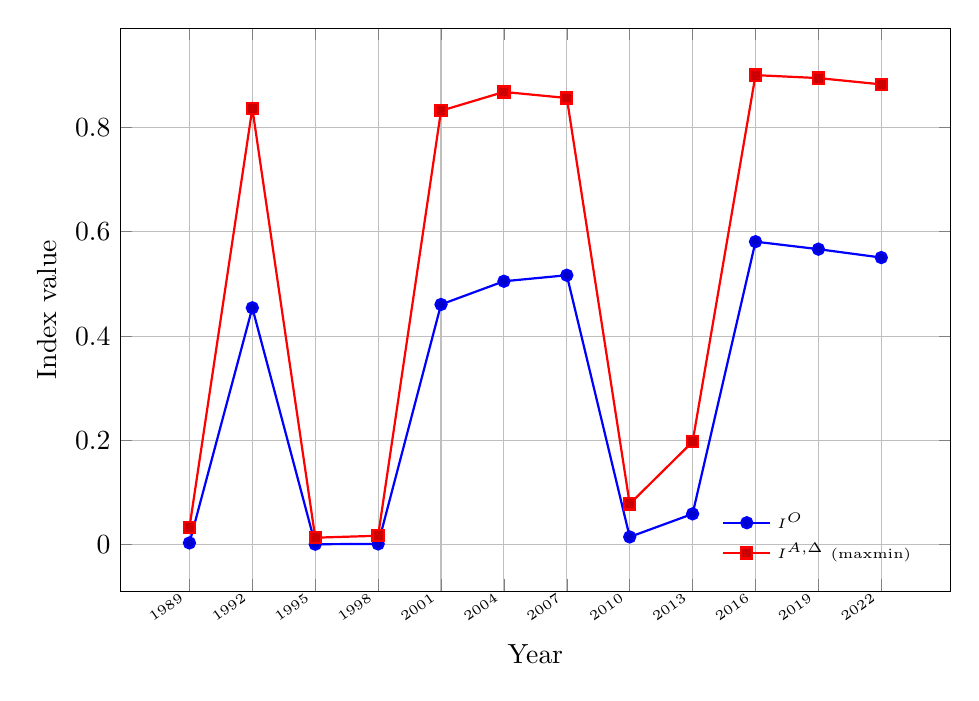
\begin{tikzpicture}
\begin{axis}[
width=\textwidth,
height=0.72\textwidth,
xlabel={Year},
ylabel={Index value},
legend pos=south east,
legend style={font=\tiny,draw=none,fill=none,cells={anchor=west}},
grid=major,
scaled x ticks=false,
xtick={1989,1992,1995,1998,2001,2004,2007,2010,2013,2016,2019,2022},
xticklabel style={/pgf/number format/fixed,/pgf/number format/precision=0,/pgf/number format/1000 sep={},rotate=35,anchor=east,font=\tiny},
]
\addplot+[thick, blue] coordinates {(1989, 0.00345679) (1992, 0.45420980) (1995, 0.00101300) (1998, 0.00151829) (2001, 0.46059219) (2004, 0.50509036) (2007, 0.51665059) (2010, 0.01492539) (2013, 0.05916722) (2016, 0.58098651) (2019, 0.56661761) (2022, 0.55052196)};
\addlegendentry{$I^{O}$}
\addplot+[thick, red] coordinates {(1989, 0.03302322) (1992, 0.83650211) (1995, 0.01352704) (1998, 0.01723812) (2001, 0.83197784) (2004, 0.86804867) (2007, 0.85641169) (2010, 0.07827416) (2013, 0.19745497) (2016, 0.90025411) (2019, 0.89458458) (2022, 0.88251198)};
\addlegendentry{$I^{A,\Delta}$ (maxmin)}
\end{axis}
\end{tikzpicture}
\end{minipage}
\hfill
\begin{minipage}[t]{0.495\textwidth}
\centering
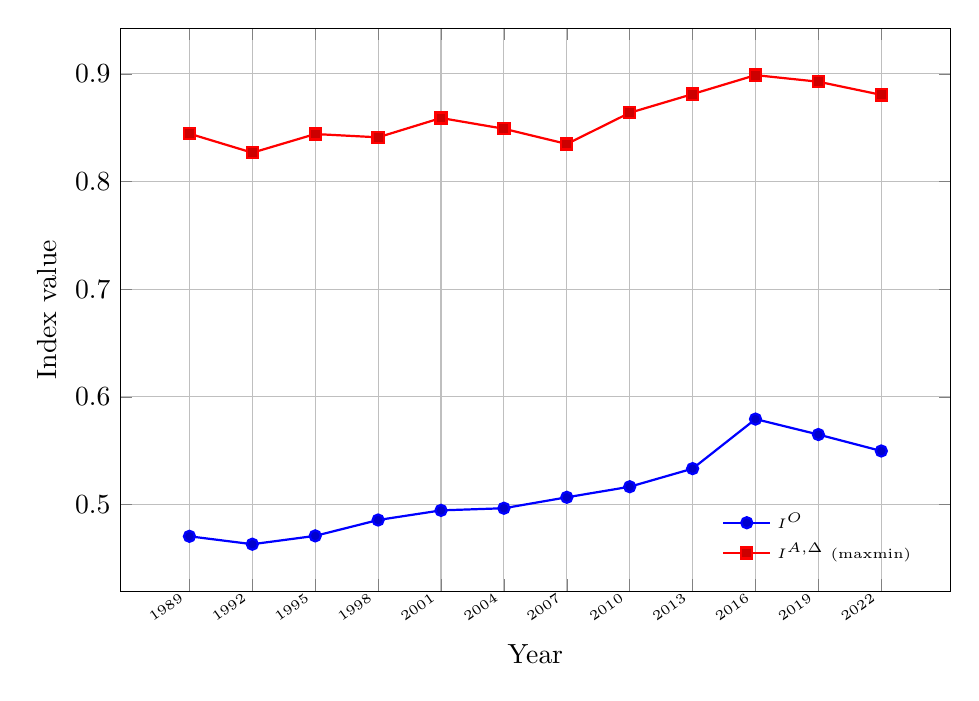
\begin{tikzpicture}
\begin{axis}[
width=\textwidth,
height=0.72\textwidth,
xlabel={Year},
ylabel={Index value},
legend pos=south east,
legend style={font=\tiny,draw=none,fill=none,cells={anchor=west}},
grid=major,
scaled x ticks=false,
xtick={1989,1992,1995,1998,2001,2004,2007,2010,2013,2016,2019,2022},
xticklabel style={/pgf/number format/fixed,/pgf/number format/precision=0,/pgf/number format/1000 sep={},rotate=35,anchor=east,font=\tiny},
]
\addplot+[thick, blue] coordinates {(1989, 0.47041226) (1992, 0.46307234) (1995, 0.47081570) (1998, 0.48555404) (2001, 0.49449629) (2004, 0.49648862) (2007, 0.50665159) (2010, 0.51645977) (2013, 0.53328392) (2016, 0.57931068) (2019, 0.56495325) (2022, 0.54967373)};
\addlegendentry{$I^{O}$}
\addplot+[thick, red] coordinates {(1989, 0.84446578) (1992, 0.82676589) (1995, 0.84413116) (1998, 0.84106348) (2001, 0.85901554) (2004, 0.84901233) (2007, 0.83488981) (2010, 0.86385187) (2013, 0.88124314) (2016, 0.89884248) (2019, 0.89272684) (2022, 0.88050806)};
\addlegendentry{$I^{A,\Delta}$ (maxmin)}
\end{axis}
\end{tikzpicture}
\end{minipage}

{\footnotesize $I^{A,\pi}$ with singleton $C=\{\pi_t\}$ equals $I^{O}$ (audit CSV: columns I\_O and I\_A\_singleton).}

% Gross Assets inequality measures
